% \pdfoutput=1    % apparently this is needed at the beginning for arXiv to process it
\documentclass[letterpaper, 10 pt, conference]{ieeeconf}

\IEEEoverridecommandlockouts                              % This command is only needed if 
                                                          % you want to use the \thanks command

\overrideIEEEmargins                                      % Needed to meet printer requirements.

% numbers option provides compact numerical references in the text. 
% \usepackage[numbers]{natbib}
\usepackage{multicol}
\usepackage[bookmarks=true]{hyperref}

% Various packages
\usepackage{float}
\usepackage{comment}
\usepackage{array}
\usepackage{graphicx}
\usepackage{booktabs}
\usepackage{multirow}
\usepackage[normalem]{ulem}
\usepackage{soul}

% Various math packages
\usepackage{amsmath}								
\usepackage{amssymb}
\usepackage{latexsym}
\usepackage{amsthm}
\usepackage{bm}
\usepackage{commath}
\usepackage{float}
\usepackage{units}

% packages for drawings
\usepackage{tikz}
% \usetikzlibrary{external}
% \tikzexternalize[prefix=tikz/] % activate!
\usetikzlibrary{arrows,shapes,trees,calc}
\usetikzlibrary{backgrounds}
\usepackage{pgfplots}
\pgfplotsset{compat=1.15}
\usepgfplotslibrary{polar}
\usepgfplotslibrary{patchplots}

% % reduce white space after captions
% \setlength{\textfloatsep}{10pt}

%% downsample images to make file smaller
%\usepackage{epstopdf}
%\epstopdfDeclareGraphicsRule{.pdf}{png}{.png}{convert #1 \OutputFile}
%\DeclareGraphicsExtensions{.png,.pdf}

% packages for 3d plotting with tikz
\usepackage{tikz-3dplot} %requires 3dplot.sty to be in same directory, or in your LaTeX installation
%\usepackage[active,tightpage]{preview}  %generates a tightly fitting border around the work
%\PreviewEnvironment{tikzpicture}
%\setlength\PreviewBorder{2mm}

% Commands for theorems
\newtheorem{definition}{Definition}[section]
\newtheorem{theorem}{Theorem}[section]
\newtheorem{assumption}{Assumption}[section]

% Definitions of custom colors
\definecolor{lightyellow}{RGB}{255,236,132}
\definecolor{lightgreen}{RGB}{161,239,10}
\definecolor{darkgreen}{RGB}{61,124,68}
\definecolor{lightblue}{RGB}{72,131,219}
\definecolor{darkblue}{RGB}{39,63,186}
\definecolor{plgreen}{RGB}{27,158,119}
\definecolor{plorange}{RGB}{217,95,2}
\definecolor{plpurple}{RGB}{117,112,179}
\definecolor{plpink}{RGB}{231,41,138}


% Editing tools
\newcounter{count}
\usepackage{color}  % For Highlighting
\newcommand{\hilight}[1]{\colorbox{yellow}{#1}}
\newcommand{\David}[1]{\textcolor{red}{(#1)}}
\newcommand{\Ram}[1]{\textcolor{blue}{\textbf{\thecount} : (#1)} \addtocounter{count}{1}}
\newcommand{\Dan}[1]{\textcolor{magenta}{(#1)}}
\newcommand{\Audrey}[1]{\textcolor{maroon}{(#1)}}

% Set macros to make certain things easier
\newcommand{\mtx}[1]{\begin{bmatrix} #1 \end{bmatrix}}
\newcommand{\aln}[1]{\begin{align} #1 \end{align}}
\newcommand{\dv}[1]{\dot{\vec{#1}}}
\newcommand{\xv}{x}
\newcommand{\uv}{u}
\newcommand{\Fv}{F}
\newcommand{\Real}{\mathbb{R}}
\newcommand{\F}{\mathcal{F}}

% Load and define stuff needed to add labels in the margins
\usepackage{marginnote}

% Set macro for labeling edits
\newcommand{\revcomment}[2]{\textcolor{red}{#2} \marginnote{\##1}} % Include reference commands
\renewcommand{\revcomment}[2]{#2}   % removes coloring of edited sections, i.e. makes doc look normal (comment this line out for highlighted edits)

% Uncomment lines below to hide comments and deleted text (to make reading easier)
% \renewcommand{\Ram}[1]{}
% \renewcommand{\sout}[1]{}

\title{\LARGE \bf
Linear System Identification of Soft Robots \\ Using Koopman Operator Theory
% Linear Identification of Nonlinear Soft Robot Systems\\ Using Koopman Theory 
}


\author{Daniel Bruder, %<-this % stops a space
        C. Cavid Remy, %
        and Ram Vasudevan, \emph{Member, IEEE} %
\thanks{*This material is supported by the Toyota Research Institute, and is based upon work supported by the National Science Foundation Graduate Research Fellowship Program under Grant No. 1256260 DGE. Any opinions, findings, and conclusions or recommendations expressed in this material are those of the author(s) and do not necessarily reflect the views of the National Science Foundation.}% <-this % stops a space
\thanks{The authors are with the Mechanical Engineering Department at the 
        University of Michigan, Ann Arbor, MI 48109, USA
        \{\tt\small bruderd, cdremy, ramv\}@umich.edu}%
% \thanks{This work has been submitted to the IEEE for possible publication. Copyright may be transferred without notice, after which this version may no longer be accessible.}
}

\begin{document}

\maketitle
\thispagestyle{empty}
\pagestyle{empty}

\begin{abstract}
%% Soft robots are difficult to model, but safe to observe
Soft robots are challenging to model due in large part to the nonlinear properties of soft materials.
Fortunately, this softness makes it possible to safely observe their behavior under random control inputs, making them amenable to large-scale data collection and system identification.
%%
This paper implements and evaluates a system identification method based on Koopman operator theory
in which models of nonlinear dynamical systems are constructed via linear regression of observed data by exploiting the fact that
every nonlinear system has a linear representation in the infinite-dimensional space of real-valued functions called observables.
% which offers a way to represent a nonlinear system as a linear system in the infinite-dimensional space of real-valued functions called observables
% and enables models of nonlinear systems to be constructed via linear regression of observed data.
%%
% The approach does not suffer from the limited convergence guarantees of other nonlinear system identification methods, which typically consist of solving a nonlinear non-convex optimization problem. 
The approach does not suffer from some of the shortcomings of other nonlinear system identification methods, which typically require the manual tuning of training parameters and have limited convergence guarantees.
%%
A dynamic model of a pneumatic soft robot arm is constructed via this method, and used to predict the behavior of the real system.
The total normalized-root-mean-square error (NRMSE) of its predictions % over twelve validation trials 
is lower than
that of several other identified models including a neural network, NLARX, nonlinear Hammerstein-Wiener, and linear state space model.
% The total normalized-root-mean-square error (NRMSE) of its predictions over twelve validation trials was 2.1\%.
% In comparison, the NRMSE of the predictions of several other identified models including a neural network, NLARX, nonlinear Hammerstein-Wiener, and linear state space model were greater than 4.4\%.








%% OLD TEXT BELOW THIS LINE 

% \David{In general I am not a fan of the structure: ``You could do A and it fails, or you could B and it fails, so here let's do C''.  Instead, I would say ``we use C to this, which doesn't suffer from the drawbacks of A and B'', C being, of course the koopman idea.  I.e., something along the lines of: ``In this paper, we propose such a sys-id based on the Koopman operator theory. This theory offers a way ...  The approach thus doesn't suffer from ....''}

% %% Nonlinear system identification is hard, linear sysid is easy
% Nonlinear system identification methods generally consist of solving optimization problems with limited convergence guarantees, therefore the resulting model may be suboptimal \David{the solution is suboptimal, the model is what? incorrect? Not the best possible description? Not sure}.
% Linear system identification, i.e. linear regression, does not suffer from this shortcoming, but linear models have shown limited ability to capture soft robot dynamics.

% %% Koopman operator theory
% Koopman operator theory offers a way to represent nonlinear systems as linear systems in the infinite dimensional space of observables.
% This enables a model of a nonlinear system to be constructed via linear regression of observed data.
% %% Contribution
% In this paper, a system identification method based on Koopman operator theory is used to construct a dynamic model of a pneumatically actuated soft robot arm.
\end{abstract}

\IEEEpeerreviewmaketitle

% Input sections here
\section{Introduction}
\label{sec:intro}

%% Soft robots can do cool things because they are compliant, but are difficult to model and control for the same reason
Soft robots, or robots that incorporate non-rigid materials into their morphology to facilitate compliant interactions with the external world, are being developed for purposes such as manipulating delicate objects, adapting to unstructured environments, and enabling safe interactions with coexisting humans \cite{rus2015design}.
While such robots demonstrate physical capabilities beyond those of traditional rigid-bodied robots, their dynamic behavior is not well-understood \cite{george2018control} \Ram{Can you cite a reference of some kind?}.
The infinite degrees of freedom and \hl{hysteretic behavior} \sout{highly nonlinear nature} of soft materials make it difficult to construct accurate models of soft robots without making significant simplifying assumptions such as constant curvature \cite{rus2015design}, quasi-static \cite{george2018control}, or simplified geometry \cite{bruder2017model} \Ram{you are only referencing a handful of papers despite having an infinite amount of space for references. This is dangerous especially since our competitors are going to review this paper and will expect to be cited..}.
These models 
% \hl{suffer from the same shortcoming as linearizations of nonlinear models in that they}
only describe behavior well in the subset of robot configurations where all assumptions hold, hence they are limited in applicability \Ram{can you describe with a more concrete example what you mean?}.
% white-box model based on first principles, e.g. a model for a physical process from the Newton equations, but in many cases such models will be overly complex and possibly even impossible to obtain in reasonable time due to the complex nature of many systems and processes

%% Lack of good models poses a problem for control
\hl{This lack of globally valid models poses a problem for control}
\sout{This poses a problem for control} \Ram{what poses a problem for control. Be specific.}.
When a good enough model is available, a predictive controller can be built that uses the model to calculate a feedforward term, then a feedback term can be added to account for minor model uncertainty and disturbances.
% stabilize around that desired point/account for model uncertainty/error (i.e. make up the difference).
However, if a good model is unavailable, feedback must be more heavily relied upon.
Since feedback is reactionary rather than anticipatory it can be slow to track a set point and prone to unwanted oscillations.
More troublingly, relying heavily on feedback to compensate for an inaccurate model has been shown to reduce the compliance of soft robotic systems \cite{della2017controlling}.
That is, excessive feedback negates the desirable compliance of a soft robot by replacing the its natural dynamics with a slower, stiffer system.
To control soft robots in a manner that reduces dependence on feedback and simultaneously preserves their compliance, better models are needed.

%% Figure: Overview Diagram
\begin{figure}[t]
    \centering
    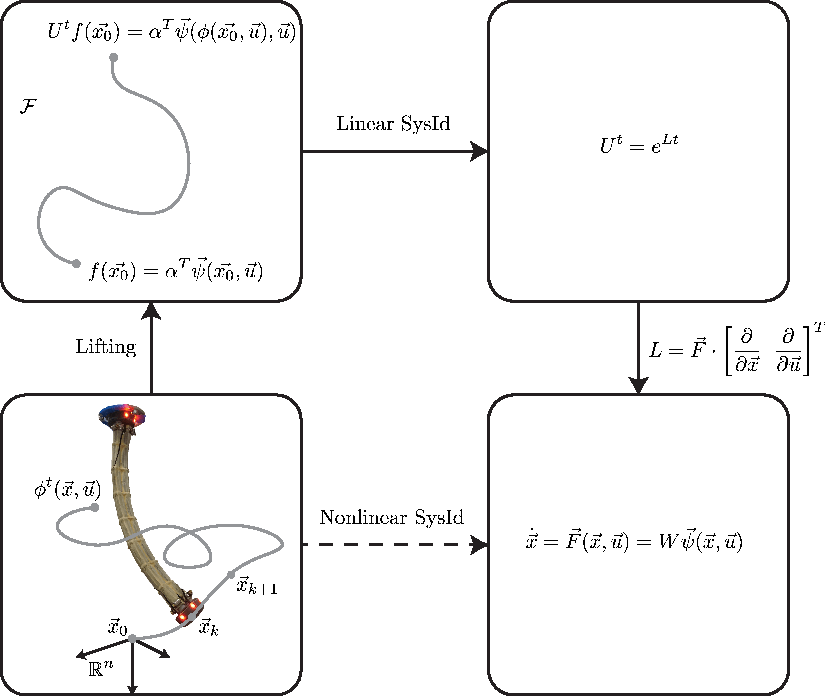
\includegraphics[width=\linewidth]{figures/overviewDiagram_rough.pdf}
    \caption{Caption: Overview of sysid method}
    \label{fig:overview}
\end{figure}

%% Soft robots are particularly well suited for system identification
\hl{Since traditional physics-based models of soft robots are typically insufficient or too complex for control, empirical models can be built instead}
\sout{White box models \Ram{what is a white box model?} for soft robots based on first principles are typically insufficient or too complex to be used for control, for the reasons stated above} \Ram{This is again a fairly sharp transition and is lacking in references.}. 
\sout{However,} By virtue of their soft bodies it is often possible to safely command arbitrary control inputs without risk of damaging a soft robot or nearby human operators.
Thus, soft robots are amenable to data collection over their entire operation range, making them particularly well suited for data-driven system identification techniques.
% Since a white-box model based on first principles, e.g. a model for a physical process from the Newton equations, are typically unavailable or too complicated to be used in control due to the complex nature of soft robots, (grey and black box models built via) system identification are needed.
%% Linear system identification is trivial
For linear systems, system identification \sout{trivially} \Ram{don't use words like trivial or intuitive. Its a mean thing to say to a reader who does not understand.} consists of fitting a linear model to observed data via linear regression, which is numerically efficient and \Dan{globally convergent?, not sure how to say this} (except in rare cases) \Ram{reference?}.
\hl{However, linear models have a limited ability to capture the dynamics of soft robots which are often characterized by their nonlinear behaviors.}
\Ram{you probably also want to say that linear system id is somehow not applicable to soft robot and cite a reference.}.
%% Nonlinear system identification is hard
For nonlinear systems, identifying a model is much more difficult since it consists of solving a nonlinear non-convex optimization problem, for which global convergence is not guaranteed \Ram{reference?}.

%% Neural network has successfully been applied to soft robot
\hl{Despite its challenges, nonlinear system identification of a soft robot has been demonstrated in the past.}
\sout{Despite its challenges, nonlinear system identification has been demonstrated successfully on soft robots in the past} \Ram{This is an awkward sentence. What does it mean to demonstrate successfully? }.
In \cite{gillespie2018learning} a Deep Neural Network (DNN) was used to model the behavior of a 1 DOF pneumatic soft robot arm.
The resulting \hl{model predictive controller} (MPC) \Ram{spell out the first time} with the neural network model acting as its predictor performed comparably to an MPC controller with a much more complicated \hl{physics-based} \sout{white box} model \Ram{make sure you define white box at some point}.
While in this case the neural network model was effective, a weakness of neural network models in general is the extent to which the training process is heuristic in nature.
A neural network model depends on the specific training parameters chosen (e.g. number of hidden layers, number of nodes per layer, activation function, termination condition), 
\hl{which must be selected through trial and error until acceptable results are achieved.}
% and training may result in a sub-optimal neural network model for a given set of data.
\Ram{be more explicit about the potential shortcomings...}

%% Koopman let's us do linear sysid (trivial) on a nonlinear system
A more reliable system identification approach utilizes Koopman operator theory to perform linear system identification of nonlinear systems \Ram{what does more reliable mean?}.
This approach relies on the idea of lifting nonlinear dynamical systems to an infinite dimensional space, where those systems have a linear representation.
\Ram{maybe these next few sentences are too much detail for now since that is something you are going to present later on...maybe just highlight its strengths? You may want to reference the figure you have developed as well.}
\sout{The Koopman Operator is a linear operator that describes the flow of observable functions of state along trajectories of the system.
By exploiting the lifting obtained through the Koopman operator,}
In this space, it is possible to describe the dynamic behavior of a system by identifying a linear operator in the space of observable functions instead of identifying a nonlinear vector field in the state space.
This linear operator, called the Koopman operator, is identified via linear regression, so it does not suffer from the indeterminacy of other nonlinear system identification methods.
% Since the Koopman operator is defined on an infinite-dimensional vector space, in practice it must be projected onto a finite basis of observable functions.
% However, with a suitably large finite dimensional approximation, we demonstrate that we can capture the true nonlinear system dynamics of a soft robot arm more accurately and more reliably than several other nonlinear system identification methods.

\Ram{I think you need a sentence here listing out the contributions of this paper....}
\Dan{I thought that's what this sentence does...}
In this paper we apply the Koopman based system identification method described in \cite{mauroy2016linear} and \cite{mauroy2017koopman} to create a dynamic model of a soft robot arm and demonstrate that it captures the system's true dynamic behavior better than the models generated by several other state-of-the-art nonlinear system identification methods including a neural network model, a nonlinear auto-regressive moving average model with exogenous inputs (NARMAX model), a nonlinear Hammerstein-Wiener model, and a state space model.

%% Why is this contribution significant?: Could enable real-time sysid/control, MPC, 
To the author's knowledge, this technique has never before been used to identify the dynamic model of a real system, much less a soft robot.
We believe that this system identification method applied to soft robots will enable the rapid development of new and effective control strategies by making accurate nonlinear dynamic models easier to construct.
% We believe that the models generated are accurate enough to be useful in control applications such as predictors in MPC controllers.
% Due to its numerical simplicity, this method also has the potential to be incorporated into real-time simultaneous sysid/control applications.

%% Outline of the rest of this paper
The rest of this paper is organized as follows:
In Section \ref{sec:theory} we formally introduce the Koopman Operator and describe the system identification method. 
In Section \ref{sec:experiment} we describe the soft robot and experimental procedure used for collecting input-output data of the system.
In Section \ref{sec:results} we summarize the results of applying various nonlinear system identification techniques to the collected data and compare the performances of the models generated. Concluding remarks and perspectives are provided in section \ref{sec:conclusion}.

\section{Koopman Operator Method for \\ System Identification}
\label{sec:theory}

%% Overview of method
This section \David{Paper?} presents \David{Or:  In this paper, we propose to use...} a method for system identification that exploits the fact that any finite-dimensional nonlinear system has an equivalent infinite-dimensional linear representation in the space of real-valued functions of the system's state and input.
In this space of real-valued functions, the (linear) Koopman operator describes the flow of functions along trajectories of the system.
The relationship between the finite and infinite dimensional representations of the system is bijective and well-defined \cite[\Ram{would be good to cite a particular theorem from this textbook}]{lasota2013chaos}.
This enables us to approximate the Koopman operator via linear regression on observed data, then extract the equivalent nonlinear system representation.
% A thorough explanation of this method can be found in \cite{mauroy2016linear} or \cite{mauroy2017koopman}.
\David{In the remainder of this section, we will summarize the ...}This section summarizes the system identification method presented in \cite{mauroy2016linear} and \cite{mauroy2017koopman} applied to system with known input. \Ram{you'll prolly want to remind the readers of the novelty in that you are doing this for a real system} \David{Agree that this would be good.  Also in the introduction.  See:  claim of contribution.}.


%% Overview of lifting technique
\subsection{Overview of Lifting Technique}


%% System representation in state space
Consider a dynamical system
\begin{align}
    \dot{x} &= \Fv(\xv,\uv)    \label{eq:nlsys}
\end{align}
where $\xv \in \Real^n$ is the state of the system, $\uv \in \Real^m$ is the input and ${F}$ is continuously differentiable in $x$.
Denote by $\phi(t,\xv_0,\uv)$ the solution to \eqref{eq:nlsys} at time $t$ when beginning with the initial condition $\xv_0$ at time $0$ and a constant input $\uv$ applied for all time between $0$ and $t$.
For simplicity, we denote this map, which is referred to as the \emph{flow map}, by $\phi^t (\xv_0, \uv)$ instead of $\phi (t, \xv_0, \uv)$.

%% System representation in the space of observables
The system can be lifted to an infinite dimensional function space $\F = L^2(X \times U, \Real)$ where $X \subset \Real^n$ and $U \subset \Real^m$ are compact subsets and $ L^2(X \times U, \Real)$ is the space of square integrable real-valued functions with domain $X \times U$.
In $\F$, the flow of the system is characterized by the semigroup \Ram{whats a semigroup? Does it matter? If so at least define it or give a reference.} of Koopman operators 
$U^t : \F \to \F$, for each $t \geq 0$,
which describes the evolution of the observables $f \in \F$ along the trajectories of the system according to the following definition:
\begin{align}
    U^t f = f \circ \phi^t      
    % && \forall f \in \F, t \geq 0
    \label{eq:koopman}
\end{align}
\Ram{Give an example of what this is or why its important. Maybe use your figure?}
As desired, $U^t$ is a linear operator even if the system \eqref{eq:nlsys} is nonlinear, since for $f_1, f_2 \in \F$ and $\lambda_1, \lambda_2 \in \Real$
\begin{align}
    \begin{split}
    U^t (\lambda_1 f_1 + \lambda_2 f_2) &= \lambda_1 f_1 \circ \phi^t + \lambda_2 f_2 \circ \phi^t \\
    &= \lambda_1 U^t f_1 + \lambda_2 U^t f_2.
    \end{split}
\end{align}
Thus the Koopman operator provides a linear representation of the system in the infinite-dimensional space of observables \cite{budivsic2012applied}. 

%% Relationship between representations of the system
One can show that there is a one-to-one correspondence between the infinite-dimensional Koopman operator and finite-dimensional vector field \Ram{cite a specific theorem from lasota}.
To understand this relationship, consider the derivative of an observable, $\dot{f}$, along trajectories of the system:
\begin{align}
\dot{f}(x,u) &= \frac{\partial f}{\partial x} \frac{dx}{dt} + \frac{\partial f}{\partial u}\frac{du}{dt} \\
           &= \frac{\partial f}{\partial x} F(x,u) \\
           &= ( F \cdot \nabla_{\xv} ) f(x,u)
\end{align}
where the second relation follows since $u$ is held constant and where $\nabla_x$ is the gradient with respect to $x$.
Since this equation holds for all observables, we introduce the infinitesimal generator $L$ \David{Isn't $L$ used to define the space of square integrable functions?}  of the Koopman operator  \cite[Section 7.6]{lasota2013chaos} which is defined as :\Ram{1. you never explain what the infinitestimal generator is...or even cite an appropriate reference. 2. it would help the reader if you described the domain and range of $L$}
\begin{align}
    % L &= \Fv \cdot \mtx{ \frac{\partial}{\partial \xv} & \frac{\partial}{\partial \uv} }^T
    L &= \Fv \cdot \nabla_{\xv}
    \label{eq:L2F}
\end{align}
Note, that one can show the following relationship between the Koopman operator and its infinitesimal generator \cite{}\Ram{cite a result}:
% where $\nabla_x$ is the gradient with respect to $x$, and $L$ is the infinitesimal generator of the Koopman operator  \cite[Section 7.6]{lasota2013chaos} \Ram{1. you never explain what the infinitestimal generator is...or even cite an appropriate reference. 2. it would help the reader if you described the domain and range of $L$} which satisfies
\begin{align}
    U^t &= e^{L t} = \sum_{k=0}^\infty \frac{t^k}{k!} L^k
    \label{eq:U2L}
\end{align}
These equations can be used to solve for the vector field $F$ when the Koopman operator $U^t$ is known \Ram{where will you show this?}.

%% Steps of sysid method
By providing a linear representation of a system with a one-to-one correspondence to its nonlinear representation, Koopman operator theory enables linear system identification of nonlinear systems. 
This process proceeds in three steps \Ram{do we want to make this an algorithm box?} \Dan{I do think so}.
In step one, measured states of the system are lifted to the space of observables.
Step two consists of performing least-squares regression on the lifted data to obtain an approximation of the Koopman operator.
In step three, the nonlinear vector field $\Fv$ is obtained via \eqref{eq:L2F} and \eqref{eq:U2L}.
The following three subsections describe each of these steps in more detail.

\begin{algorithm}
\SetAlgoLined
\KwResult{Write here the result }
 initialization\;
 \While{While condition}{
  instructions\;
  \eIf{condition}{
   instructions1\;
   instructions2\;
   }{
   instructions3\;
  }
 }
 \caption{How to write algorithms}
\end{algorithm}


%% STEP 1: Lifting the Data
\subsection{Step 1: Lifting the Data}   \label{sec:step1}

%% Overview of this step
The first step of the Koopman based system identification method consists of converting empirical data into a form that can be used to identify a linear model in the space of observables.
Theoretically this process would consist of ``lifting'' state measurements into the infinite-dimensional space of observables $\F$.
In the implementation, however, measurements can only be lifted into a finite-dimensional subspace.
%% Approximation must be finite dimensional=
Define $\F_N \subset \F$ to be the subspace of $\F$ spanned by $N$ linearly independent basis functions $\{ \psi_k \}_{k=1}^N$ 
\Ram{maybe give us an example of an appropriate set?}.
%
Any observable ${f \in \F_N}$ can be written as a linear combination of elements of its basis
\begin{align}
    f &= \alpha_1 \psi_{1} + \cdots + \alpha_N \psi_N.
\end{align}
Note that the vector of coefficients ${\alpha = \mtx{\alpha_1 & \cdots & \alpha_N}^T}$ provide a \emph{vector representation} for any $f \in \F_N$.
To evaluate $f$ at a given state $\xv$ and constant input $\uv$, we introduce the \emph{lifting function} ${\psi}:\Real^n \times \Real^m \to \Real^N$ defined as:
\begin{align}
    {\psi}(\xv, \uv) = \mtx{ \psi_1(\xv, \uv) & \cdots & \psi_N(\xv, \uv)}^T
    \label{eq:lift}
\end{align}
Then, $f(\xv, \uv)$ can be expressed in vector form as
\begin{align}
    f(\xv, \uv) &= {\alpha}^T {\psi}(\xv, \uv).
    \label{eq:fxu}
\end{align}
We refer to ${\psi}(\xv, \uv)$ as an N-dimensional ``lifted'' version of ${(\xv, \uv)}$, since multiplying ${\psi}(\xv, \uv)$ by the vector representation of an observable yields the value of the observable at $\xv, \uv$.



%% STEP 2: Approximating the Koopman Operator
\subsection{Step 2: Approximating the Koopman Operator} \label{sec:step2}

The second step of the Koopman-based system identification method is to identify the Koopman operator that best describes the flow of the lifted versions of measured data points.
While the Koopman operator is theoretically infinite-dimensional, for practical purposes we identify a finite-dimensional approximation of it in $\F_N$ which we denote by $\bar{U}^t$ \David{I would propose to use a consistent notation for your finite dimensional approximations.  Either with the bar or with $_N$}.
Note, that $\bar{U}^t$ can be represented by an $N \times N$ matrix which operates on observables via matrix multiplication:
\begin{align}
    \bar{U}^t {\alpha} &= {\beta} 
    % && {\alpha}, {\beta} \in \F_N .
    \label{eq:Ubar}
\end{align}
where $\alpha, \beta$ are vector representations of observables in $\F_N$.
Our goal is to find a $\bar{U}^t$ that describes the action of the infinite dimensional Koopman operator $U^t$ as accurately as possible in the $L^2$-norm sense on the finite dimensional subspace $\F_N$  of all observables.
% We want to find $\bar{U}^t$ such that it describes the action of the infinite-dimensional Koopman operator $U^t$ as accurately as possible, i.e.
% \begin{align}
%     U^t f(\xv,\uv) &\approx ( \bar{U}^t {\alpha} )^T {\psi}(\xv, \uv)
% \end{align}
% \hl{for all $f \in \F_n$ with $\alpha$ as its vector representation}.
% From \eqref{eq:koopman}, the Koopman operator describes the flow of observables in $\F$.
Therefore, to perfectly mimic the action of $U^t$ acting on an observable in $\F_N \subset \F$, the following should be true
\begin{align}
    ( \bar{U}^t {\alpha} )^T {\psi}(\xv, \uv) &=
    {\alpha}^T {\psi} \left( \phi^t(\xv,\uv), \uv \right).
    \label{eq:Ubar}
\end{align}
Since this is just a linear equation, to find the best approximation of the finite dimensional Koopman operator in the $L^2$-norm sense, we let  ${\psi}^\dagger$ denotes the least-squares pseudoinverse of ${\psi}$ and let: \David{???}
It then follows that for a given ${x \in \Real^n, \uv \in \Real^m}$ solving \eqref{eq:Ubar} for $\bar{U}^t$ yields the best possible approximation of $U^t$ on $\F_N$
\begin{align}
    \bar{U}^t = \left( {\psi}(\xv, \uv)^T \right)^\dagger {\psi}( \phi^t(\xv,\uv), \uv )^T.
    \label{eq:Uapprox}
\end{align}

%% this whole paragraph should be removed...
% \sout{
% From \eqref{eq:koopman}, \eqref{eq:fxu}, and \eqref{eq:Ubar} we can approximate the effect of applying the infinite-dimensional Koopman operator $U^t$ to some $f \in \F_N$ using its finite-dimensional projection
% % \begin{align}
% %     U^t f(\xv,\uv) &\approx ( \bar{U}^t {\alphapeolpe} )^T {\psi}(\xv, \uv) =
% %     {\alpha}^T {\psi} \left( \phi^t(\xv,\uv), \uv \right) \\
% %     \label{eq:Utfapprox}
% % \end{align}
% where $\alpha$ is the vector representation of $f$.
% \Ram{you probably want to explain why each of these equations follow and I really hate when things are written down with approximations like that since with approximations without any explanation as to why its approximate.}
% From this relation the projection of the Koopman operator can be approximated
% % \begin{align}
% %     \bar{U}^t &\approx \left( {\psi}(\xv, \uv)^T \right)^\dagger {\psi}( \phi^t(\xv,\uv), \uv )^T
% %     \label{eq:Uapprox}
% % \end{align}
% where ${\psi}^\dagger$ denotes the pseudoinverse of ${\psi}$ \Ram{Same comment as earlier.}.
% }


%% How this is done on our system
To approximate the Koopman operator from experimental data, we take $K+1$ discrete state measurements with sampling period $T_s$. Under the assumption that the control input is constant between samples, we separate the data into a set of $K$ so-called ``snapshot pairs'' of the form ${ \{(\xv_k,\uv_k),(\xv_{k+1},\uv_k)\} \in \Real^{(n \times m) \times 2} }$ where
\begin{align}
    x_{k+1} &= \phi^{T_s} (x_k, u_k).
\end{align}
For our basis of $\F_N$, we choose the basis of monomials of $\xv$ and $\uv$ with total degree less than or equal to $w$, which implies $N=(n+m+w)!/\left((n+m)!w!\right)$ \cite[\Ram{cite a specific definition or result}]{mauroy2016linear}. 
We then lift all of the snapshot pairs according to \eqref{eq:lift} and compile them into the following $K \times N$ matrices
\begin{align}
    &\Psi_x = \mtx{ {\psi}(\xv_1, \uv_1)^T \\ \vdots \\  {\psi}(\xv_K, \uv_K)^T}
    &&\Psi_y = \mtx{ {\psi}(\xv_2, \uv_1)^T \\ \vdots \\  {\psi}(\xv_{K+1}, \uv_{K})^T}
\end{align}
 $\bar{U}^{T_s}$ is chosen so that it yields the least squares best fit to all of the observed data, which, following from \eqref{eq:Uapprox}, is given by 
\begin{align}
    \bar{U}^{T_s} &:= \Psi_x^\dagger \Psi_y
\end{align}
where ${\Psi}^\dagger$ denotes the least-squares pseudoinverse of ${\Psi}$.


%% STEP 3: Obtaining the vector field
\subsection{Step 3: Obtaining the Vector Field} \label{sec:step3}

The final step of the Koopman-based system identification method is to identify the nonlinear vector field by making use of the one-to-one correspondence between the infinite and finite dimensional system representations.
% Consider again the vector field $\Fv(\xv,\uv)=\mtx{F_1(\xv,\uv) & \cdots & F_n(\xv,\uv)}^T$.
% Each $F_i$ is a function of state and input that can be represented as a linear combination of the basis elements of $\F$.
As earlier, our goal is to find a $\bar{F}$ that describes the behavior of the vector field $F$ as accurately as possible in the $L^2$-norm sense on the finite dimensional subspace $\F_N$.

% Our goal is to find a $\bar{U}^t$ that describes the action of the infinite dimensional Koopman operator $U^t$ as accurately as possible in the $L^2$-norm sense on the finite dimensional subspace $\F_N$  of all observables.

% As we did earlier, we restrict ourselves to represent $F$ using elements from the finite-dimensional subspace $\F_N$. 
% In particular, our goal is to find a finite dimensional representation 

% matrix of coefficients $C \in \Real^{n \times N}$ to 
% % \begin{align}
% %     C &= \mtx{ c_{1,1} & \cdots & c_{1,N} \\ \vdots & \ddots & \vdots \\ c_{n,1} & \cdots & c_{n,N} }
% %     \label{eq:C}
% % \end{align}

% the vector field resulting from this system identification method is only a linear combination of the basis elements of $\F_N$:
% \begin{align}
%     \Fv(\xv, \uv) &\approx C {\psi}(\xv, \uv)
%     \label{eq:F2C}
% \end{align}
% where $C$ is an $n \times N$ matrix of coefficients
% \begin{align}
%     C &= \mtx{ c_{1,1} & \cdots & c_{1,N} \\ \vdots & \ddots & \vdots \\ c_{n,1} & \cdots & c_{n,N} }
%     \label{eq:C}
% \end{align}
% Therefore, identifying the vector field reduces to the task of identifying $nN$ total coefficients $c_{i,j}$.

The vector field is related to the Koopman operator through its infinitesimal generator \Ram{reference a specific equation}.
% \Ram{sharp transition between the previous paragraph and the ensuing one}
With the approximation of the Koopman operator $\bar{U}^{T_s}$ found in Section \ref{sec:step2}, we can solve for the infinitesimal generator of the Koopman semigroup $\bar{L}$ by inverting \eqref{eq:U2L}
\begin{align}
    \bar{L} &= \frac{1}{T_s} \log{ \bar{U}^t } \in \Real^{N \times N}
\end{align}
where $\log$ denotes the principal matrix logarithm \cite[\Ram{cite a particular equation}]{higham2008functions}.
Note that the principal matrix logarithm is only defined for matrices whose eigenvalues all have non-negative real components, and that $\bar{U}^t$ may have zero or negative eigenvalues when the number of data points is too small \cite{mauroy2016linear}.
Therefore this method might fail if the number of data points is insufficient.
In this instance, more system measurements must be taken to resolve this issue.

With $\bar{L}$ known, \eqref{eq:L2F} can be used to identify $\bar{F}$.
Consider $L$ applied to an observable $f \in \F_N$.
According to \eqref{eq:L2F}, this is equivalent to the inner product of the vector field $\Fv$ and the gradient of $f$ with respect to $x$  
\begin{align}
    L f(\xv,\uv) &= \frac{\partial f(\xv,\uv)}{\partial \xv} \Fv(\xv,\uv).
    \label{eq:L2Fxu}
\end{align}
\Dan{i.e. the dynamics of the observable $\partial f / \partial t$}
Let $\alpha \in \Real^N$ be the vector representation of $f$.
Then from \eqref{eq:fxu} the finite-dimensional equivalent of \eqref{eq:L2Fxu} is given by
\begin{align}
    (\bar{L} {\alpha})^T \vac{\psi}(\xv,\uv) &= {\alpha}^T \frac{\partial \psi(\xv, \uv)}{\partial \xv} \bar{F}.
    \label{eq:Lbar2C}
\end{align}
We seek the vector field $\bar{F}$ such that \eqref{eq:Lbar2C} holds as well as possible in the $L^2$-norm sense for all observed data.
Therefore we choose the least-square solution to \eqref{eq:Lbar2C} over the set of all observed data points $\left\{ (x_k,u_k) | k = 1,...,K \right\}$ which is given by
\begin{align}
    \bar{F} &= \mtx{ \frac{\partial \psi(\xv_1, \uv_1)}{\partial \xv} \\ \vdots \\ \frac{\partial \psi(\xv_K, \uv_K)}{\partial \xv} }^\dagger
    \mtx{ \bar{L}^T & \cdots & 0 \\ \vdots & \ddots & \vdots \\ 0 & \cdots & \bar{L}^T }
    \mtx{ \psi(x_1,u_1) \\ \vdots \\ \psi(x_K,u_K) }.
\end{align}
% \begin{align}
%     \bar{F} &\approx \mtx{ \frac{\partial \psi(\xv_1, \uv_1)}{\partial \xv} \\ \vdots \\ \frac{\partial \psi(\xv_K, \uv_K)}{\partial \xv} }^\dagger
%         \mtx{ \bar{L}^T \\ \vdots \\ \bar{L}^T }.
% \end{align}
For a more thorough treatment of this process, see \cite{mauroy2016linear, mauroy2017koopman}.
\section{System Identification of a Soft Robot}
\label{sec:experiment}

To demonstrate and evaluate the performance of the method outlined in Section \ref{sec:theory}, we applied it to a continuously deformable soft robot arm and compared the resulting model to those generated by several other nonlinear system identification techniques.
In the following, we describe in detail the robotic hardware, experimental setup, measurement procedure, and the data processing involved in the system identification process, as well as the process by which performance was evaluated and compared across models.
% \David{In the following, we explain in detail the used robotic hardware, experimental setup, measurement proces, ...}This section describes the composition of the robot and recount the setup, measurement, and data pre-proccessing involved in the system identification process.


\subsection{Hardware Description}

The soft robot used in this experiment consisted of three pneumatically driven McKibben actuators (also known as Pneumatic Artificial Muscles or PAMs) adhered together by latex rubber and connected to a common base mount on one end and to an end effector on the other (see Fig. \ref{fig:flaccy}).
During the trials, the pressure inside each actuator was varied using a pneumatic pressure regulator {(Enfield TR-010-g10-s)}, and the displacement and velocity of the end effector was measured at $60 \text{Hz}$ using a commercial motion capture system (Phase Space Impulse X2E).

%% state space representation of model
For this robot, it is our primary interest to control the motion of the end effector.
% \David{Try to use more declarative language.  We have discussed this in the past.  Other people do a lot of different things (and might disagree in your notion of primary interest), but you can simply say what your interest is: ``Our declared control goal for this setup is to dynamically control the kinematic motion of ...} With robotic manipulators, it is often of primary interest to dynamically control the motion of the end effector.
% \David{To this end, we chose...} 
Hence, we chose a state representation of the system which is capable of describing the dynamics of the end effector as an ordinary differential equation, namely the position and velocity of the end effector with respect to a global coordinate frame, as shown in Fig.~\ref{fig:flaccy}
% Hence, we chose to represent the state of our soft robot as the position and velocity of the end effector with respect to a global coordinate frame, as shown in Fig. \ref{fig:flaccy}
\begin{align}
    \vec{x} &= \mtx{ x_1 & x_2 & x_3 & \dot{x}_1 & \dot{x}_2 & \dot{x}_3 }^T
    \label{eq:state}
\end{align}
% It is worth noting that our chosen set of state variables may not be rich enough to uniquely describe the actual state of the system, e.g. there may be multiple body configurations associated with the same end effector location.
% In this case, the learned models will provide a best approximation of the dynamics of the chosen variables based on the training data, but won't satisfy the formal requirements of a state-space model.

\subsection{Randomized Control Input}

To generate a representative sampling of the system's behavior over its entire operation range, a randomized input was applied.
The control input into the system $\uv$ was a set of three $0-10 \text{V}$ signals into the pressure regulators corresponding to actuator pressures of $\approx 0-140 \text{ kPa}$
\aln{
    \uv (t) &= \mtx{ u_1 (t) & u_2 (t) & u_3 (t) }^T,   && u_i \in [0,10]
}
Before each trial, a $3 \times K_u$ table $\Upsilon$ of uniformly distributed random numbers between zero and ten was generated to be used as an input lookup table.
$K_u$ was chosen to be large enough to provide inputs over the entire length of each trial.
Each control input was smoothly varied between elements in consecutive columns of the table over a transition period $T_u$ with a time offset of $T_u / 3$ between each of the three control signals,
\aln{
    u_i (t) &= \frac{(\Upsilon_{i,k+1} - \Upsilon_{i,k})}{T_u} \left( t + \frac{(i-1) T_u}{3} \right) + \Upsilon_{i,k}
    \label{eq:input}
}
where $k = \text{floor}\left( {t} / {T_u} \right)$ is the current index into the lookup table at time $t$. 
% (see Fig. \ref{fig:randInput}).

%% Figure: Randomized Inputs
% \begin{figure}
%     \centering
%     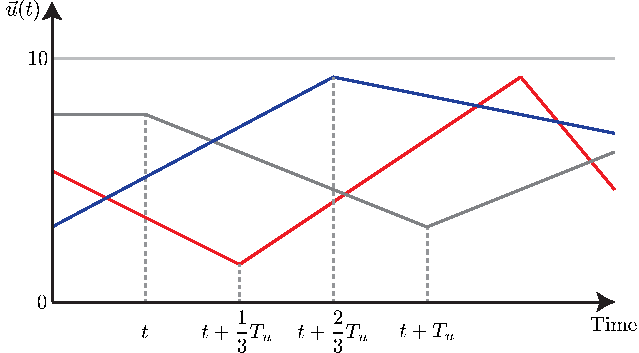
\includegraphics[width=\linewidth]{figures/randInput3dim.pdf}
%     \caption{Caption: Randomized control inputs \David{I would add the dotted line at t+4/3T.}}
%     \label{fig:randInput}
% \end{figure}


\subsection{Data Collection}

% %% TABLE: Trial parameters
% \begin{table}[h]
%     \centering
%     \caption{Data Collection Parameters}
%     \begin{tabular}{|c||c|c|}
%         \hline
%          & $\bm{T_u}$ \textbf{(s)} & \textbf{Length (min)} \\
%         \hline
%          Trial 1 & 3 & 40:06 \\
%          Trial 2 & 3.5 & 31:26 \\
%          Trial 3 & 4 & 8:16 \\
%          Trial 4 & 5 & 26:09 \\
%          Trial 5 & 5 & 28:38 \\
%          Trial 6 & 8 & 31:35 \\
%         \hline
%     \end{tabular}
%     \label{tab:trialParams}
% \end{table}

%% TABLE: RMSE results table
\begin{table}
    \rowcolors{2}{white}{gray!25}
    \setlength\tabcolsep{5pt} % default value: 6pt
    \centering
    \caption{Data Collection Parameters}
    \begin{tabular}{|c|c|c|c|c|c|c|}
        \hline
        \rowcolor{white} 
        & \multicolumn{6}{c |}{\textbf{Trial}} \\
        \hhline{~------} \rowcolor{white}
        \multirow{-2}{*}{} & $1$ & $2$ & $3$ & $4$ & $5$ & $6$ \\
        \hline
        % RESULTS FOR ROBOT A
        \textbf{Length (min)}     &  40:06  &  31:26  &  8:16  &  26:09  &  28:38  &  31:35 \\
        \textbf{$\bm{T_u}$ (s)}  &  3.0  &  3.5  &  4  &  5  &  5  &  8 \\
        \hline
        % % RESULTS FOR ROBOT B
        % \cellcolor{white} & Koopman & & & & & & & & \\
        % \cellcolor{white} & Neural Net & & & & & & & & \\
        % \cellcolor{white} & State Space & & & & & & & & \\
        % \cellcolor{white} & Ham.-Weiner & & & & & & & & \\
        % \multirow{-5}{*}{\cellcolor{white} \rotatebox[origin=c]{90}{\textbf{Robot B}}}
        % & NLARX & & & & & & & & \\
        % \hline
    \end{tabular}
    \label{tab:trialParams}
\end{table}

%% TABLE: Trial parameters (ONLY IF TWO ROBOTS ARE USED)
% \begin{table}[h]
%     \centering
%     \caption{Data Collection Parameters}
%     \begin{tabular}{|c||c|c||c|c|}
%         \hline
%         & \multicolumn{2}{c|}{Robot A} & \multicolumn{2}{c|}{Robot B} \\
%         \hline
%          & $\bm{T_u}$ \textbf{(s)} & \textbf{Length (min)} & $\bm{T_u}$ \textbf{(s)} & \textbf{Length (min)} \\
%         \hline
%          Trial 1 & 3   & 40:06 & 2   & \\
%          Trial 2 & 3.5 & 31:26 & 3   & \\
%          Trial 3 & 4   & 8:16  & 3.5 & \\
%          Trial 4 & 5   & 26:09 & 4   & \\
%          Trial 5 & 5   & 28:38 & 5   & \\
%          Trial 6 & 8   & 31:35 & 6   & \\
%         \hline
%     \end{tabular}
%     \label{tab:trialParams2}
% \end{table}

Data collection proceeded in 6 trials each lasting an average of $\approx27$ minutes.
The input transition period $T_u$ varied from trial to trial, taking values between 3 and 8 seconds (see Table~\ref{tab:trialParams} for the specific values for each trial).
% The specific testing parameters for each trial can be found in Table \ref{tab:trialParams}.
After collecting data, raw position and velocity measurements were put through a moving average filter with window size of $1$s to reduce noise, then sampled uniformly with a period $T_s = 0.02$ seconds.
Sampled velocity measurements were put through a second moving average filter with window size of $1$ second due to the higher noise content of the velocity signal.
%% Partitioning of trail data into training and validation sets
The time-series data from each trial was partitioned into training and validation sets. 
Three 10 second validation sets were extracted from each trial and the remainder of the trial data was used for training.

%% FIGURE: Showing what flaccy looks like
\begin{figure}
    \centering
    \vspace{10pt}
    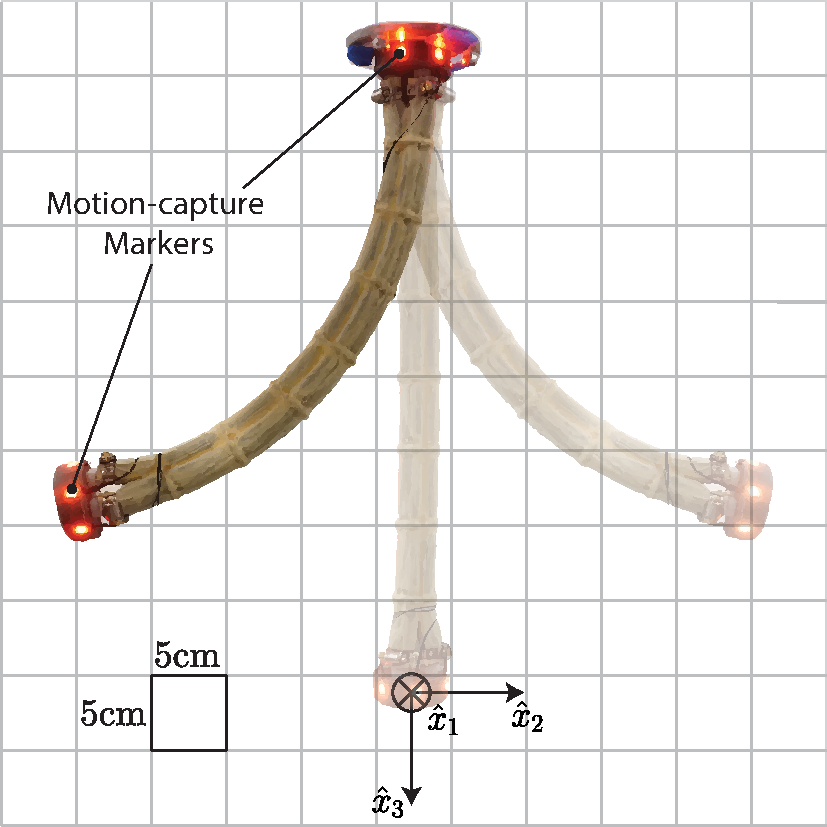
\includegraphics[width=0.8\linewidth]{figures/flaccyDiagram_bothways_v4.pdf}
    \caption{System identification was performed on a soft robot consisting of three PAMs adhered together. 
        Active motion capture markers on the base and end effector enabled tracking of the position and velocity of the end effector relative to the fixed global coordinate frame marked by unit vectors $\hat{x}_1,\hat{x}_2,\hat{x}_3$ where $\hat{x}_1$ is pointing into the page. The robot's range of motion given control inputs defined in \eqref{eq:input} is depicted.}
    \label{fig:flaccy}
\end{figure}


%% Model Comparison
\subsection{Model Comparison}
\label{sec:modelcomparison}

%% Performance was evaluated by comparing simulations to real measurements
We generated a state space model from the technique described in section \ref{sec:theory} using a monomial basis of maximum degree $w=3$ and the collected training data.
We then evaluated its accuracy by comparing model simulations to each of the validation data sets (Fig.~\ref{fig:koopmanSim}).
Goodness of fit for the trajectory of a state $y$ was calculated using the normalized root-mean-square error (NRMSE), defined:
%% Normalized Root Mean-Square Error
\aln{
    \text{RMSE} &= \sqrt{ \frac{\sum_{k=1}^{N_\text{total}} \left( y_k - \hat{y}_k \right)^2}{N_\text{total}} } \\
    \text{NRMSE} &= \left( \frac{\text{RMSE}}{y_\text{max} - y_\text{min}} \right) \cdot 100 \%
    % 1 - \frac{ \| y - \hat{y}  \| }{ \| y - \text{mean}(y) \| }
}
where $\hat{y}$ is the simulated value of the state, $N_\text{total}$ is the total number of points, and $y_{\text{min/max}}$ are the measured minimum/maximum values of the state observed over all trials.

%% For comparison, other sysid methods were also used on the same set of data
The performance of our model was benchmarked against a linear state space, nonlinear Hammerstein-Wiener, nonlinear auto-regressive with exogenous inputs (NLARX), and a feedforward neural network model.
The models were trained and evaluated on the non-lifted time-series data from the experiments described in Section \ref{sec:experiment}, and generated using either the Matlab System Identification Toolbox or Neural Network Toolbox \cite{MATLAB:2017}.
The state space model was generated using the subspace method \cite[Chapter 7]{ljung1987system} and specified to be 6 dimensional, i.e. the same dimension as the state defined in \ref{eq:state}.
The neural network model was trained using the Levenberg-Marquardt backpropogation algorithm and sigmoid activation functions.
It was trained several times using combinations of 10-30 hidden neurons and 1-10 delays.
Only the results for the best of these models, corresponding to 10 hidden neurons and 10 delays, is displayed in Fig. \ref{fig:comparison} and Table \ref{tab:RMSE}.
\section{Results}
\label{sec:results}

The model generated by the Koopman system identification method has a total RMSE averaged across position states and velocity states of {5.98~mm} and {3.66~mm/s}, respectively.
As shown in Table \ref{tab:RMSE}, this corresponds to a total NRMSE averaged across all states of 2.1\%. 
By this metric, it performs more than twice as well as the best competing linear and nonlinear models which have average NRMSEs of 4.6\% and 4.5\%, respectively (see Fig.~\ref{fig:comparison}).
% Fig. \ref{fig:comparison} shows the NRMSE of each model over all states and all trials as compared to the validation data.
The Koopman model also exhibits the smallest standard deviation of the NRMSE across states.
This implies that the Koopman model more consistently captures the real behavior of all six states of the system, rather than just a subset of them.
Fig. \ref{fig:koopmanSim} illustrates the ability of the Koopman-based model to predict the position of the end effector over a 30 second time horizon.

% \David{I feel your results should start with what is obvious to you: IT WORKS. It converges.  You get a result. The result can predict behavior with an accuracy of XYZ.  It took x long to get this result.  If you used different seeds, you always get the same answer (because linear fitting).  Don't forget that you are doing this for the first time and it is important to note that it works.  People will ask themselves how well it works and how they can use it.  Do you need to tune stuff?  Do you need to carefully select parameters or initial guesses?}
% \David{Can you quantify the level of `non-linearity' of your robot?  This would be very valuable for a reader who wants to understand if this nonlinear approach is even necessary.  Can you discuss which of the other methods are linear/ nonlinear.}


%% FIGURE: Koopman simulation plot
\begin{figure}
    \centering
    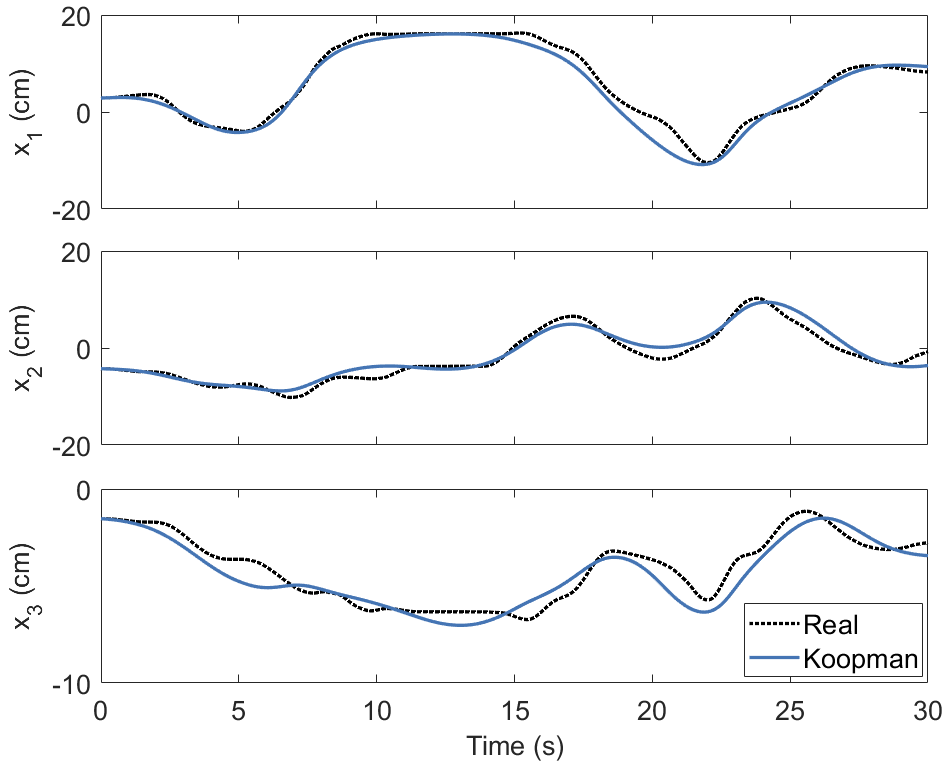
\includegraphics[width=0.9\linewidth]{figures/koopPlot4_cropped.png}
    \caption{
    The measured position of the robot end effector over a 30 second time window (black,dotted) superimposed with the position predicted by the Koopman-based model (blue) given the same initial condition and control inputs. Coordinates are defined with respect to the global coordinate frame depicted in Fig. \ref{fig:flaccy}.}
    \label{fig:koopmanSim}
\end{figure}

%% FIGURE: Comparison bar graph
\begin{figure}
    \centering
    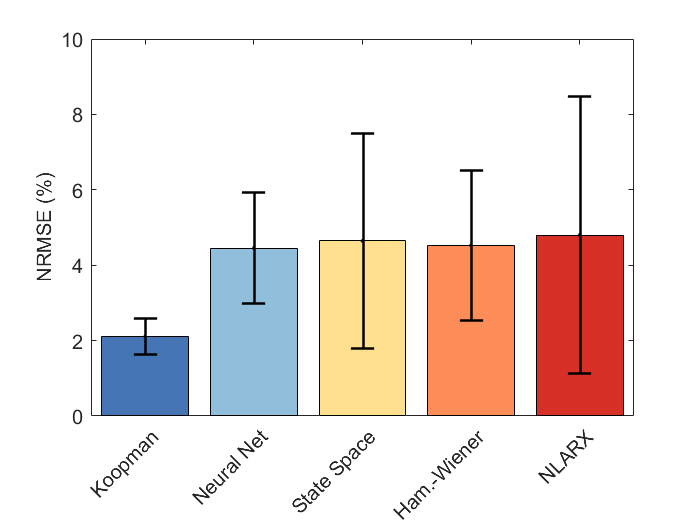
\includegraphics[width=\linewidth]{figures/NRMSE2.png}
    \caption{Shown is the total NRMSE averaged across all states for each of the models, with the standard deviation designated by the black bar. The average NRMSE of the Koopman-based model is less than half of that of the other models, with a standard deviation of less than one third of the other models.}
    \label{fig:comparison}
\end{figure}

%% TABLE: RMSE results table
\begin{table}
    \rowcolors{2}{white}{gray!25}
    \setlength\tabcolsep{5pt} % default value: 6pt
    \centering
    \caption{Total NRMSE (\%) over all validation trials}
    \begin{tabular}{|c|c|c|c|c|c|c|c|c|}
        \hline
        \rowcolor{white} 
        & \multicolumn{6}{c |}{\textbf{States}} & & \textbf{Std.} \\
        \hhline{~------~~} \rowcolor{white}
        \multirow{-2}{*}{\textbf{Model}} & $x_1$ & $x_2$ & $x_3$ & $x_4$ & $x_5$ & $x_6$ & \multirow{-2}{*}{\textbf{Avg.}} & \textbf{Dev.} \\
        \hline
        % RESULTS FOR ROBOT A
        Koopman     &  2.4  &  2.0  &  2.9  &  1.7  &  1.5  &  2.0 & 2.1 & 0.5 \\
        Neural Net  &  5.8  &  4.0  &  6.6  &  3.9  &  2.8  &  3.5 & 4.5 & 1.5 \\
        State Space &  5.1  &  3.1  &  9.9  &  3.0  &  1.8  &  4.8 & 4.6 & 2.9 \\
        Ham.-Weiner &  7.0  &  4.5  &  6.9  &  3.0  &  2.3  &  3.1 & 4.5 & 2.0 \\
        % \multirow{-5}{*}{\cellcolor{white} \rotatebox[origin=c]{90}{\textbf{Robot A}}}
        NLARX       &  5.0  &  3.0 &  12.0  &  3.8  &  2.1  &  2.8 & 4.8 & 3.7 \\
        \hline
        % % RESULTS FOR ROBOT B
        % \cellcolor{white} & Koopman & & & & & & & & \\
        % \cellcolor{white} & Neural Net & & & & & & & & \\
        % \cellcolor{white} & State Space & & & & & & & & \\
        % \cellcolor{white} & Ham.-Weiner & & & & & & & & \\
        % \multirow{-5}{*}{\cellcolor{white} \rotatebox[origin=c]{90}{\textbf{Robot B}}}
        % & NLARX & & & & & & & & \\
        % \hline
    \end{tabular}
    \label{tab:RMSE}
\end{table}
\section{Conclusion}
\label{sec:conclusion}

%% Summary of what we've shown
We have successfully applied a system identification technique based on Koopman operator theory to a soft robot, and shown that the model generated outperforms those generated by other state-of-the-art nonlinear system identification methods. \David{expand lightly use last paragraph of results}

\David{New paragraph, discussing reasons for success}
Linear system identification of this nonlinear systems is possible by exploiting the fact that nonlinear systems have linear representations in the infinite dimensional space of observables.
Even though in practice it is intractable to identify an infinite-dimensional model, by identifying the projection of the model on a sufficiently high-dimensional subspace of observables, we can recover an approximate model of the nonlinear system that still captures its behavior.

\David{I would discuss the numerical challenges.}

%% Future work / remaining challenges
Soft robots are notoriously difficult to model, but uniquely safe to observe under arbitrary control inputs.\David{Not a challenge of your approach.  Repeat of goal.}
Thus system identification is an ideal choice for modeling them.\David{not a challenge}
This paper demonstrates the potential of Koopman operator theory to improve upon existing system identification methods for soft robots.\David{not a challenge}
Future work will generalize this approach to higher dimensional models, non-polynomial models, and models that account for external loading and contact forces. \David{expand.  Discuss challenges.}

\David{wrap up with positive outlook and take home message..}

% %% Why this is important/significant
% That's not all...
% Koopman system identification is well suited for identification of dynamic models for soft robots
% The potential applications of this lifting technique are far reaching.
% The linear system representation could be leveraged for control



% %% Future possibilities


% Predictors for MPC, observers, simultaneous control and system identification, adaptive control (like an arm that picks something up and immediately updates it's model of itself...)


% \addtolength{\textheight}{-12cm}   % This command serves to balance the column lengths
%                                   % on the last page of the document manually. It shortens
%                                   % the textheight of the last page by a suitable amount.
%                                   % This command does not take effect until the next page
%                                   % so it should come on the page before the last. Make
%                                   % sure that you do not shorten the textheight too much.

% \input{sections/acknowledgement.tex}


\bibliographystyle{IEEEtran}
\bibliography{references}


\end{document}


